\section{Connected Dominating Set for Surface Triangulations}
\label{bounded_genus}
In this section, we establish \cref{genus_result}, the extension of \cref{main_result2} to surface triangulations of genus $g = o(n)$.
Briefly, a \defin{surface or 2-manifold} $\mathcal{S}$ is a compact connected Hausdorff topological space such that every point in $\mathcal{S}$ is locally homeomorphic to the plane i.e. it has a neighbourhood homeomorphic to $\mathbb{R}^2$. Every such surface can be created from the sphere $\mathbb{S}^2$, by adding handles and cross-caps. The \defin{Euler genus} of a surface with $h$ handles and $c$ cross-caps is $2h+c$.
% define surfaces related info
%Briefly, a \defin{surface or 2-manifold} $\mathcal{S}$ is a compact connected Hausdorff topological space such that every point in $\mathcal{S}$ is locally homeomorphic to the plane i.e. it has a neighbourhood homeomorphic to $\mathbb{R}^2$. The genus $g$ of a surface $\mathcal{S}$ is the number of handles or cross-caps added to the sphere $\mathbb{S}^2 = \{x \in \mathbb{R}^3 : ||x||= 1\}$ to form a surface homeomorphic to $\mathcal{S}$. In the former case, we call the surface $\mathcal{S}_g$, and the later case we call it $\mathcal{N}_g$. A surface is \defin{orientable} if it is homeomorphic to $\mathcal{S}_g$ for some non-negative $g$, we say it is \defin{non-orientable} if it is homeomorphic to a surface $\mathcal{N}_g$ for some positive $g$. The Euler-genus $\Bar{g}$ of a surface $\mathcal{S}$ is equal to $2g$ if $\mathcal{S}$ is orientable and $g$ if $\mathcal{S}$ is non-orientable. For a detailed account on graph and surfaces, we refer the reader to \cite{mohar2001graphs, lee2010introduction}.\pat{Consider using Euler genus:  The Euler genus of a surface with $h$ handles and $c$ crosscaps is $2h + c$.}

% \begin{patnote}
%    Briefly, a \defin{surface or 2-manifold} $\mathcal{S}$ is a compact connected Hausdorff topological space such that every point in $\mathcal{S}$ is locally homeomorphic to the plane i.e. it has a neighbourhood homeomorphic to $\mathbb{R}^2$. Every such surface can created from the sphere $\mathbb{S}^2$, by adding handles and cross-caps. The \defin{Euler genus} of a surface with $h$ handles and $c$ cross-caps is $2h+c$.
    % The genus $g$ of a surface $\mathcal{S}$ is the number of handles or cross-caps added to the sphere $\mathbb{S}^2 = \{x \in \mathbb{R}^3 : ||x||= 1\}$ to form a surface homeomorphic to $\mathcal{S}$. In the former case, we call the surface $\mathcal{S}_g$, and the later case we call it $\mathcal{N}_g$. A surface is \defin{orientable} if it is homeomorphic to $\mathcal{S}_g$ for some non-negative $g$, we say it is \defin{non-orientable} if it is homeomorphic to a surface $\mathcal{N}_g$ for some positive $g$. The Euler-genus $\Bar{g}$ of a surface $\mathcal{S}$ is equal to $2g$ if $\mathcal{S}$ is orientable and $g$ if $\mathcal{S}$ is non-orientable. For a detailed account on graph and surfaces, we refer the reader to \cite{mohar2001graphs, lee2010introduction}.\pat{Consider using Euler genus:  The Euler genus of a surface with $h$ handles and $c$ crosscaps is $2h + c$.} \hussein{add the definition for sigma too}
% \end{patnote}
% \hussein{I think, we should omit the discussion about oriantability as now the new theorem works on any surface in contrast to the previous one!!}

%%% define embedding related information
We follow the definitions given in \citet[Appendix~B]{diestel:graph}. An \defin{arc}, a \defin{circle}, and a \defin{disc} in a surface $\mathcal{S}$, is a subsets of $\mathcal{S}$ that is homeomorphic to $[0, 1]$, to a unit circle $\mathbb{S}^1 = \{x \in \mathbb{R}^1: ||x|| = 1\}$, or to a unit disc $\mathbb{B}^2 = \{x \in \mathbb{R}^2 : ||x|| < 1\}$, respectively. 
% A closed disk is a disk that contains its boundary.  
The set of all arcs in $\mathcal{S}$ is denoted by $A_\mathcal{S}$. 
% \hussein{each arc in S is a subset of S; there is a kind of redandency.} \pat{Sure, but a point in $\mathcal{S}$ is a different kind of object than an arc in $\mathcal{S}$. Vertices map to point of $S$ and edges map to arcs.}
An \defin{embedding} of a graph $G$ in a surface $\mathcal{S}$ is a map \defin{$\sigma: V(G)\cup E(G) \longrightarrow \mathcal{S}\cup A_\mathcal{S}$} that sends vertices of $G$ to distinct points in $\mathcal{S}$ and sends an edge $xy$ to 
% an $\sigma(x)-\sigma(y)$ arc in $\mathcal{S}$\pat{Suggested rewrite: 
an arc $\sigma(xy)$ in $\mathcal{S}$ with endpoints $\sigma(x)$ and $\sigma(y)$ in such a way that interior of $\sigma(xy)$ is disjoint from $\{\sigma(v):v\in V(G)\}$ and from the interior of $\sigma(vw)$ for every $vw\in E(G)\setminus\{xy\}$.  For a subgraph $Z$ of $G$, we call $\sigma(Z):=\{\sigma(v):v\in V(X)\}\cup \bigcup_{vw\in E(X)}\sigma(vw)$ the \defin{embedded subgraph} $Z$.
% where no inner points of this arc intersects another arc or an image of a vertex. We let $\sigma(G):=\{\sigma(v):v\in V(G)\}\cup \bigcup_{e\in E(G)}\sigma(e)$.  
A graph $G$ equipped with an embedding $\sigma$ on a surface $\mathcal{S}$ is called an \defin{$\mathcal{S}$-embedded} graph. A \defin{face} of $G$ in $\mathcal{S}$ is a component of $\mathcal{S} \setminus \sigma(G)$.  
% In this context, we call $\sigma(vw)$ the \defin{embedded edge} $vw$.


The \defin{surface-map} $\Sigma$ of an $\mathcal{S}$-embedded graph $G$ is a tuple $(V, E, F)$ where $V$ is the set of vertices, $E$ is the set of edges, and $F$ is the set of faces in the embedding $\sigma$ of $G$. We call a surface-map a \defin{surface triangulation} if every face in $F$ is a disc in $\mathcal{S}$ whose boundary is an embedded $3$-cycle of $G$.  The \defin{Euler genus} of a surface triangulation $\Sigma$ is the Euler genus of the surface $\mathcal{S}$.
% \hussein{I think this is better because if our embedding of $G$ has every face is a disk, then it works, I guess.} \pat{Good, let's just leave it defined for surface triangulations then.}
%\hussein{ok, we can double check here \url{https://jeffe.cs.illinois.edu/teaching/comptop/2023/notes/19-surface-maps.pdf}} \pat{I don't think there's anything to check. Euler's formula tells us exactly the number of edges in a surface triangulation, as a function of $n$ and $g$.  If there were a smaller genus surface on which we could embed $G$ then we would get a contradiction.}
% \hussein{I think we should talk about the surface with minimum genus, because $\Sigma$ can be planar but embedded on higher surface; I think saying $\Sigma$ is maximal triangulation could work, but not sure}. \pat{I think it's the case that the graph of a surface-triangulation has the same genus as the surface (because every triangle is a disk in the surface).  Let me check.  Actually, it doesn't matter because the theorem refers to a genus-$g$ surface triangulation.} \hussein{here $\Sigma$ is ambiguous it can be a planar graph for example...} \pat{But if you embed a planar triangulation on a higher genus surface, then one of its faces will not be a disc, so you don't get a surface triangulation.}
% \hussein{yes I agree, so when it is maximal triangulation, I guess we are fine but our letter $\Sigma$ does not refer to a triangulation but to a surface-map, the first sentence in the paragraph...!!} \pat{That's ok. The surface map is defined with respect to an underlying surface $\mathcal{S}$.  It's actually instructions for making $\mathcal{S}$ by gluing together faces, so it's ok to call the genus of $\Sigma$ the genus of $\mathcal{S}$.} \hussein{that is fine, I am thinking of it as data-structure for the embedded graph rather than a simplical complex...} 

% \pat{This isn't needed if we use Euler genus: The \defin{orientable genus} and the \defin{non-orientable genus} of a graph $G$ is the minimum $g$ and the minimum $g'$ such that $G$ has an embedding into surface $\mathcal{S}_g$, or $\mathcal{N}_{g'}$ respectively.  The genus of the surface-map is the genus of the underlying graph. Similarly, we define the Euler-genus of a graph and a surface-map.}
% \pat{Using Euler genus would simplify this to a single sentence.}


% A \defin{cut graph} of a map $\Sigma$ on a surace $S$ is any subgraph $X$ of $\Sigma$ such that $S \setminus X$ an open topological disk. ($\setminus$ means to remove the points from from $S$, not deleting the edges from the map).

As in \cite{EricksonNotes}, \defin{slicing} a surface map $\Sigma$ along a subgraph $Z \subseteq G$ with at least one edge produces a new map $\Sigma \bbslash Z$ which contains $\deg_{Z}(v)$ copies of every vertex $v$ of $Z$, two copies of every edge of $Z$, and at least one new face in addition to the faces of $\Sigma$.  (See \cref{slicing}.)
% \pat{I find this confusing, because a slicing produces a new graph and a new embedding of this graph, but a surface-map just refers to a set of vertices, edges, and faces.  Also, $\Sigma\bbslash Z$ contains every vertex of $G$ with $\deg_X(v)=0$.} 
The faces of $\Sigma \bbslash Z$ that are not faces of $\Sigma$ are called \defin{holes} that are missing from the surface. A \defin{planarizing subgraph} of $\Sigma$ is any subgraph $Z \subseteq G$ such that the surface-map obtained after slicing along $Z$ has genus $0$ with one or more boundary cycles \cite{EricksonNotes}.  A key property of the slicing operation is the following:  If vertices $v'$ and $w'$ are on the boundary of the same hole in $\Sigma\bbslash Z$, then the corresponding vertices $v$ and $w$ of $\Sigma$ are in the same component of $Z$. We use of the following theorem of \citet{10.5555/644108.644208}.


\begin{figure}
    \begin{center}
        \begin{tabular}{cc}
            \includegraphics[width=.45\textwidth,page=2]{figs/slicing-orig} &
            \includegraphics[width=.45\textwidth,page=4]{figs/slicing-orig} \\
            $\Sigma$ & $\Sigma\bbslash Z$
        \end{tabular}
    \end{center}
    \caption{Slicing a surface map $\Sigma$ along a subgraph $Z$ (in red). Holes in $\Sigma\bbslash Z$ are shown in black and hole boundaries are red.}
    \label{slicing}
\end{figure}

%is embedded on a closed disk with holes, consequently in the plane. 
% \pat{I don't think this is quite true.  If $Z$ contains  contractible cycles, then the surface underlying $\Sigma\bbslash Z$ is disconnected, but a closed disc with holes is connected.  The proof of \cref{Eppstein} does not make any effort to avoid contractible cycles in $Z$.  I think $X$ is a planarizing subgraph of $G$ if each component of $\mathcal{S}\setminus \sigma(X)$ is homeomorphic to a disc, possibly with holes.} \hussein{I fix it, there is something called cut graph that leaves a closed disk, but planarriser is not a cut graph but cut graph is a planariser.}
% \hussein{Should I cite the lecture notes for this paragraph?} \pat{Yes}
% A cycle is \defin{non-contractible} if it is not homotopic to a point (or nullhomotopic) i.e it cannot continuously deformed to a point in $\Sigma$.
%\pat{The preceding paragraph talks about the new surface $\Sigma'$ that we get by cutting along $C$, but doesn't explain the new graph $G'$ that we get (which now has two copies of each vertex and edge of $C$).  Maybe you want to separate the description of cutting a surface $\Sigma$ along a closed curve $C$ from the description of cutting a $\Sigma$-embedded graph $G$ along a curve $C$ that contains some vertices and edges of $G$ (but doesn't cross any edge of $G$).  This might make it easier to explain what happens when you cut $G$ along more than one cycle.}
% Then, we define the topology on the modified set as follow. Let $N$ be any strip neighbourhood of $C$ in $S$, and put $X' := \{x' | x\in C\}$ and $X'' := \{x'' | x \in C\}$. If $N$ is a cylinder, then $N \setminus C$ has two components $N'$ and $N''$, and choose the neighbourhoods of the new points $x'$ and $x''$ in $S'$ so that $X'$ and $X''$ becomes a boundary circle of $N'$ and $N''$ in $S'$, respectively, and $N' \cup X'$ and $N'' \cup X''$ become disjoint cylinders in $S'$. Finally, we turn $S'$ into a surface by capping its holes by taking two disjoint disk and identifying their boundary circles with $X'$, and $X''$ respectively.
% The \pat{orientable?} \defin{genus} of a graph $G$ is the minimum positive integer $g$ such that $G$ can be embedded on a surface of genus $g$.
%%% TODO: 
% 1. define the embedding correctly. ok 
% 2. define the genus of a graph . ok 
% 3. define a non-seperating cycle. ok 
% 4. define a slicing ok.
% 5. maybe I will add a figure.
\begin{thm}[\citet{10.5555/644108.644208}]\label{Eppstein}
Every surface triangulation $\Sigma$ with $n$ vertices and Euler-genus $g < n$ has a planarizing subgraph $Z$ with $O(\sqrt{gn})$ vertices and edges, which can be computed in $O(n)$ time.
\end{thm}

We can now prove the main result of this section, which readily establishes \cref{genus_result}.

\begin{lem}\label{generic_surface_thm}
    Let $f:\mathbb{N} \longrightarrow \mathbb{N}$ be a non-decreasing function such that every $n$-vertex (planar) triangulation has a connected dominating set of size at most $f(n)$. Then every $n$-vertex Euler genus-$g$ surface triangulation $\Sigma$ has a connected dominating set of size at most $f(n + O(\sqrt{gn})) + O(\sqrt{gn})$.
\end{lem}

\begin{proof}
Let $\Sigma:=(V,E,F)$ and let $G$ be the graph with vertex set $V$ and edge set $E$.
By applying Theorem \ref{Eppstein}, we obtain a planarizing graph
$Z$ of $\Sigma$. Treat $\Sigma \bbslash Z$ as a plane graph and add a set $E'$ of edges to obtain a planar triangulation $G'$ that has $n+O(\sqrt{gn})$ vertices. By assumption, $G'$ has a connected dominating set $X'$ whose size is at most $f(n + O(\sqrt{gn}))$.

The connected dominating set $X'$ contains vertices of $G$ and vertices of $\Sigma\bbslash Z$ that do not appear in $G$.  (These latter vertices are copies of vertices of $Z$.) To obtain a connected dominating set $X$ for $G$, we set $X:=(X'\cap V(G))\cup V(Z)$.   We now show that $X$ satisfies the requirements of the lemma.
\begin{itemize}
    \item \emph{$X$ is a dominating set:} Since $X'$ is a dominating set of $G'$, each vertex $w\in V(G)\setminus X$ is adjacent, in $G'$, to some vertex $v'\in X'$.  If $v'\in V(G)$ then $v'\in X$.  If $v'\in V(G')\setminus V(G)$, then $v'$ is a copy of some vertex $v$ of $Z$, in which case $v\in X$. In either case $w$ has neighbour, in $G$, that is contained in $X$.  Thus, $X$ is a dominating set of $G$.

    \item \emph{$G[X]$ is connected:} Let $v$ and $w$ be any two vertices in $X$. Then each of $v$ and $w$ has at at least one corresponding vertex $v'$ and $w'$, respectively, in $G'$.   Since $X'$ is a connected dominating set of $G'$, there exists a path $P':=v',z_0,\ldots,z_r,w'$ in $G'$ such that $z_0,\ldots,z_r$ is path in $G'[X']$.  If $P'$ does not contain any edge of $E'$ then $P'$ has a corresponding path in $G[X]$, so $v$ and $w$ are in the same component of $G[X]$.  If some edge $x'y'$ of $P'$ is in $E'$ then $x'$ and $y'$ are on the boundary of the same hole in $\Sigma\bbslash Z$.  Then $x'$ and $y'$ are copies of two vertices $x$ and $y$ of $G$ that are contained in the same component of $Z$.  In this case, we can replace the edge $x'y'$ with a path, in $Z$, from $x$ to $y$.  Doing this for each edge of $P'$ that is in $E'$ shows that there is a walk in $G[X]$ from $v$ to $w$, for each pair $v,w\in X$. Therefore $G[X]$ is connected.
    
    \item \emph{$X$ has size $f(n + O(\sqrt{gn}))+O(\sqrt{gn})$:} The size of $X$ is at most $|X'| + |V(Z)|\le f(n + O(\sqrt{gn})) + O(\sqrt{gn})$.
\end{itemize}
Therefore, $X$ is a connected dominating set of $G$ of size at most $f(n+O(\sqrt{gn}))+ O(\sqrt{gn})$.
\end{proof}

% \begin{thm} \label{surf_result}
% For every $n\ge 3$, every surface triangulation $\Sigma$ with $n$ vertices and genus $g = o(n)$ has a connected dominating set $X$ of size at most $10n/21 + O(\sqrt{gn})$.
% \end{thm}
\begin{proof}[Proof of \cref{genus_result}]
    By \cref{main_result2}, we can apply \cref{generic_surface_thm} with $f(n)= 10n/21$. We obtain a connected dominating set of size at most $10 (n + O(\sqrt{gn}))/21 + O(\sqrt{gn}) = 10n/21 + O(\sqrt{gn})$.  The equivalent statement about spanning trees follows from \cref{main_theorem_cor}.
\end{proof}

% \begin{proof}
% Let $\Sigma:=(V,E,F)$ and let $G$ be the graph with vertex set $V$ and edge set $E$.
% By applying Theorem \ref{Eppstein}, we obtain a planarizing graph
% % \pat{minimal planarizing graph is not defined or discussed. Maybe just say, above, that a minimal planarizing graph has no degree-$1$ vertices.}\hussein{I mentioned this in the last paragraph, I will see how I change it ...} 
% $Z$ of $\Sigma$.  Treat $\Sigma \bbslash Z$ as a plane graph and add a set $E'$ of edges to obtain a planar triangulation $G'$ that has $n:=n+O(\sqrt{gn})$ vertices.
% % obtained from performing the slicing along $Z$, we obtain a planar triangulation. 
% % Denote by $E'$ the edges used to triangulate the holes of $\Sigma \bbslash Z$. 
% Apply \cref{main_result2} to $G'$, to obtain a connected dominating set $X'$ of $G'$ whose size is at most $10n'/21+O(1)=10n/21+O(\sqrt{gn})$.

% The connected dominating set $X'$ contains vertices of $G$ and vertices of $\Sigma\bbslash Z$ that do not appear in $G$.  (These latter vertices are copies of vertices of $Z$.) To obtain a connected dominating set $X$ for $G$, we set $X:=(X'\cap V(G))\cup V(Z)$.   We claim that $X$ satisfies the requirements of the lemma.
% \begin{itemize}
%     \item \emph{$X$ is a dominating set:} Since $X'$ is a dominating set of $G'$, each vertex $w\in V(G)\setminus X$ is adjacent, in $G'$, to some vertex $v'\in X'$.  If $v'\in V(G)$ then $v'\in X$.  If $v'\in V(G')\setminus V(G)$, then $v'$ is a copy of some vertex $v$ of $Z$, in which case $v\in X$. In either case $w$ has neighbour, in $G$, that is contained in $X$.  Thus, $X$ is a dominating set of $G$.

%     \item \emph{$G[X]$ is connected:} Let $v$ and $w$ be any two vertices in $X$. Then each of $v$ and $w$ has at at least one corresponding vertex $v'$ and $w'$, respectively, in $G'$.   Since $X'$ is a connected dominating set of $G'$, there exists a path $P':=v',z_0,\ldots,z_r,w'$ in $G'$ such that $z_0,\ldots,z_r$ is path in $G'[X']$.  If $P'$ does not contain any edge of $E'$ then $P'$ has a corresponding path in $G[X]$, so $v$ and $w$ are in the same component of $G[X]$.  If some edge $x'y'$ of $P'$ is in $E'$ then $x'$ and $y'$ are on the same hole in $\Sigma\bbslash Z$.  Then $x'$ and $y'$ are copies of two vertices $x$ and $y$ of $G$ that are contained in the same component of $Z$.  In this case, we can replace the edge $x'y'$ with a path, in $Z$, from $x$ to $y$.  Doing this for each edge of $P'$ that is in $E'$ shows that there is a walk in $G[X]$ from $v$ to $w$, for each pair $v,w\in X$. Therefore $G[X]$ is connected.
    
%     \item \emph{$X$ has size $10n/21+O(\sqrt{gn})$:} The size of $X$ is at most $|X'| + |V(Z)|\le 10n'/21 + O(\sqrt{gn}) \le 10n/21 + O(\sqrt{gn})$.
% \end{itemize}
% Therefore, $X$ is a connected dominating set of $G$ of size at most $10n/21+ O(\sqrt{gn})$.
% \end{proof}
% % add to $X'$ the vertices of $Z$ after deleting the edges in $E'$ and undoing the slicing along $Z$. 



% By adding the vertices in $Z$, we ensure that every vertex that was dominated through an edge in $E'$ is in the dominating set. Thus, $X$ is a dominating set of $G$.  It remains to prove that $G[X]$ is connected. We have the following cases.  If $z \in Z \cap X'$ then nothing to proof. If $z \in Z$ is dominated by a vertex $x' \in X'$ then $z$ still adjacent to $x'$ in $X'$. Otherwise, $z \in Z$ was dominated by $z' \in Z$, then $z$ and $z'$ are connected by a path in $Z$ after adding $Z$ to $X'$; $Z$ will never be an isolated vertex since $Z$ is minimal. If $Z$ is minimal, then it doesn't have any vertices of degree less than $1$, since removing a degree-$1$ or less vertex $Z$ corresponds to gluing together two adjacent edges on a hole in $\Sigma\bbslash Z$ or gluing the space at that point. It remains to bound the size of $X$.

%  $$|X| = |X'| + |V(Z)|,$$
%  $$|X| \leq \frac{10 n'}{21} + c\sqrt{gn},$$
%  $$|X| \leq \frac{10 (n + c\sqrt{gn})}{21} + c\sqrt{gn},$$
%  $$|X| \leq \frac{10n}{21} + (\frac{10}{21} + 1)c\sqrt{gn}.$$

%  Thus,
% $$|X| = \frac{10n}{21} + O(\sqrt{gn})$$
% as desired.

% \begin{patnote}
%   I think this result can be made stronger (with a simpler proof) using the following theorem (see Page 3 here \url{https://jeffe.cs.illinois.edu/teaching/comptop/2023/notes/22-planarization.pdf}):

%   \begin{thm}
%       Every surface triangulation $\Sigma$ with $n$ vertices and Euler genus $g<n$ has a planarizing
% subgraph $Z$ with $O(\sqrt{gn})$ vertices and edges, which can be computed in $O(n)$ time.
%   \end{thm}

  

%   Here, \defin{planarizing subgraph} means that if we cut the surface $\Sigma$ along each edge of $Z$, then the resulting surface $\Sigma\bbslash Z$ is homeomorphic to a disk with holes.  Alternatively, if we start with all the individual triangular faces and glue two faces $xyz$ and $yxw$ together along their shared edge $xy$ if and only if $xy\not\in E(Z)$ then the surface we get is homeomorphic to a disk with holes.  Notice that, if $Z$ is minimal, then it doesn't have any vertices of degree $1$, since removing a degree-$1$ vertex $Z$ corresponds to gluing together two adjacent edges on a hole in $\Sigma\bbslash Z$.

%   If we call $G$ the triangulation that is embedded in $\Sigma$, then we get a graph $G'$ where each edge of $Z$ appears twice and each vertex $v\in V(X)$ appears $\deg_X(v)$ times.  So the graph $G'$ has $n':=n+O(\sqrt{gn})$ vertices. Now add edges to triangulate $G'$ and apply \cref{main_result2} to get a connected dominating set $X'$ of $G'$ of size $10n'/21=10n/21 + O(\sqrt{gn})$.  Then set  $X:=X'\cup V(Z)$ to get a connected dominating set of $G$ that has size $10n/21 + O(\sqrt{gn})$. 

%   Advantages: We get a result for $g$ up to $o(n)$ and it works for Euler genus, orientable or non-orientable.
% \end{patnote}

% \hussein{1. Define Cut Graph. 2. Epstein Theorem. 3. Rephrase theorem 6}


% \begin{patnote}
% We can go over the proof of this result tomorrow.  Erickson's notes are basically his explanation of Section 5 in this paper: \url{https://dl.acm.org/doi/pdf/10.5555/644108.644208}.  The separator $Z$ consists of 
% \begin{compactitem}
%     \item BFS layers $i+ak$ for some $i\in\{0,\ldots,k-1\}$ and all $a\in\mathbb{N}$, where $k\approx\sqrt{n/g}$;  
%     \item plus $O(g)$ paths $P_1,\ldots,P_{r}$ where each path $P_j$ has both endpoints in layer $i+ak$ and is contained in layers $i+ak,\ldots,i+(a+1)k-1$, for some integer $a$.
% \end{compactitem}
% \end{patnote}


% In order to prove Theorem \ref{surf_result}, we will use the following lemmas. 
% \begin{lem}[\cite{doi:10.1137/0401020}\label{noncont}]
%   Every n-vertex triangulation of an orientable surface $\Sigma$ of genus $g > 0$ has a non-separating cycle of length at most $O(\sqrt{n})$.
% \end{lem}
% Notice that Lemma \ref{noncont} implies Lemma \ref{to_g_zero}.
% \begin{lem}{\cite{doi:10.1137/0401020}\cite{GILBERT1984391}}\label{to_g_zero}
%     Any embedded triangulation $G$ with $n$ vertices and genus $g$ can be transformed into a genus-$0$ graph by cutting along $g$ cycles of total length $O(g\sqrt{n})$.
% \end{lem}


% \begin{proof}[Proof of Theorem \ref{surf_result}]
%     We will proceed by induction on the genus $g$. The base case follows immediately from Theorem \ref{main_result2}. Assume the results holds for triangulation of surfaces of genus $< g$. By Lemma \ref{noncont}, we have a non-contractible non-seperating cycle $C$ of length at most $O(\sqrt{n})$. The graph $G \setminus \setminus C$ has two copies of $C$, denote these cycles by $C^{\flat}$ and $C^{\sharp}$. For each of these cycles create a corresponding closed disk $D^{\flat}$  and $D^{\sharp}$. Then, identify the boundary of $D^{\flat}$ to the cycle $C^{\flat}$, similarly for $D^{\sharp}$. Next, add edges in faces bounded by $D^{\flat}$ and $D^\sharp$ so our graph $G\setminus\setminus C$ triangulates the surface obtained by slicing through $C$. Notice that the new surface has genus $< g$. Thus, we are home by induction, and we have connected dominating set of size at most $\frac{10 (n + |C|)}{21} + (g - 1) \sqrt{n + |C|}$. Now, consider the graph obtained by removing the edges inside $D^\flat$ and $D^{\sharp}$ and  gluing the cycles $C^\flat$ and $C^\sharp$. Observe, that some vertices of $C^{\flat}$ and $C^{\sharp}$ may not be dominated anymore. Thus, we add them to the new dominating set. The total size of the new dominating set is $\frac{10 (n + |C|)}{21} + (g - 1) \sqrt{n + |C|} + \sqrt{n} - |C|$.
% \end{proof}

% \pat{There is an issue here in that it's not clear what it means two cut $G$ along two (or more) $C_1$ and $C_2$ if $C_1$ and $C_2$ intersect.  If we cut along $C_1$ first to get a graph $G_1$, then $C_2$ is not a cycle in the embedded graph $G_1$ since it contains consecutive vertices $x'$ and $x''$ with no edge between them.}


% \begin{proof}[Proof of Theorem \ref{surf_result}]
% Using Lemma \ref{to_g_zero}, we transform the graph $G$ to a graph $G'$ of genus zero, by cutting through a set of non-separating cycles $\mathcal{C}$ of size $g$. Then, we triangulate every face of $G'$.\pat{I think you should say here that the only non-triangular faces of $G'$ come from the caps that were glued on when cutting $G'$.} Thus, $G'$ became planar triangulation and Theorem \ref{main_result2} applies. Let $X'$ be the obtained dominating set of size at most $\frac{10|G'|}{21}$. To obtain a dominating set $X$ for $G$, we add to $X$ the vertices of the cycles in $\mathcal{C}$. It is immediate to verify that $X$ is connected, every vertex in a cycle $C \in \mathcal{C}$ is either in $X'$ or adjacent to a vertex in $X'$. It remains to bound the size of $X$.
% $$|X| = |X'| + |\bigcup_{C \in \mathcal{C}} V(C)|,$$
% $$|X| \leq \frac{10 |G'|}{21} + cg\sqrt{|G|},$$
% $$|X| \leq \frac{10 (n + cg\sqrt{n})}{21} + cg\sqrt{n},$$
% $$|X| \leq \frac{10n}{21} + (\frac{10}{21} + 1)cg\sqrt{n}.$$

% Thus,
% $$|X| = \frac{10n}{21} + O(cg\sqrt{n})$$
% as desired.
 
% \end{proof}


% A \defin{non-separating cycle} $C$ of a graph $G$ that is embedded on a surface $\Sigma$, is a cycle of $G$ whose removal leaves $G$ connected, in addition its embedding $\sigma(C)$ is a non-separating \emph{circle} in $\Sigma$.


% A \defin{non-separating circle} $C$ in $\Sigma$ such that $\Sigma \setminus C$ has one \defin{component}, an arc connected topological space. \defin{Cutting} $\Sigma$ along a \emph{non-separating} circle $C$, in a surface $\Sigma \neq \mathbb{S}^2$, is to create a new space $\Sigma'$ from $\Sigma$ by replacing every point $x \in C$ with two points $x',x''$. Then, consider any strip neighbourhood $N$ of $C$ in $\Sigma$, and let $X' := \{x' : x\in C\}$ and $X'' := \{x'' : x \in C\}$. Since $\Sigma$ is orientable, $N$ is a cylinder and $N\setminus C$ has two components $N'$ and $N''$ and we define their boundary circles to be $X'$ and $X''$, respectively. To turn $\Sigma'$ into a surface, we cap its holes by taking two disks disjoint from $\Sigma$ and identifying their boundary circles with $X'$, and $X''$ respectively. 